\documentclass[]{article}
\usepackage{mathrsfs}
\usepackage{amsmath}
\usepackage{amsfonts}
\usepackage{graphicx}
\usepackage[left=20mm, right=20mm, top=20mm, bottom=20mm]{geometry}

\begin{document}
\huge Numeros complejos.
\\
\\
\Large Definición de un numero complejo.
\normalsize
\\
\\
Para empezar a hablar de numeros complejos primero hay que definir a la unidad imaginaria.
$$
\sqrt{-1} = i
$$
Todos los numeros de la forma $bi$ donde $b \in \mathbb{R}$ son numeros puramente imaginario.

Un numero complejo es la suma entre un numero real y uno imaginario y se suelen llamar $z$ tal que:
$$
z=a+bi
$$
Con $a \in \mathbb{R}$, $b \in \mathbb{R} $ y $z \in \mathbb{C}$
\\
\\
\Large Representación geometrica en el plano complejo
\normalsize
\\
\\
Los complejos pueden representarse en un plano mediante pares ordenados de numeros reales, esto se debe al isomorfismo que tiene $(\mathbb{C},+)$ con $(\mathbb{R}^{2},+)$ por lo tanto pueden representarse como vectores.

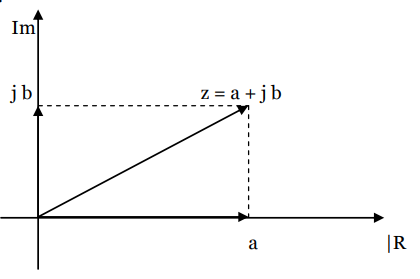
\includegraphics{../../../Imagenes/Superior/Complejos/Complejos01.PNG}


\Large Igualdad.
\normalsize
\\
\\
La igualdad entre numeros complejos se define asi:
$$
z_1 = a+bi \hspace{5pt}\wedge\hspace{5pt} z_2=c+di
$$
$$
z_1 = z_2 \Leftrightarrow a = c \hspace{5pt}\wedge\hspace{5pt} b = d
$$

\Large Modulo.
\normalsize
\\
\\
Geometricamente es el modulo del vector asociado a $z$.
$$
|z| = \sqrt{a^{2}+b^{2}}
$$

\Large Adición.
\normalsize
\\
\\
$$
z = z_1 +z_2 = a+bi + c+di = a+c+bi+di = (a+c) + (b+d) i
$$
Es equivalente a la suma de vectores, por lo tanto tiene sus mismas propiedades.
\Large Multiplicación.
\normalsize
\\
\\
$$
z = z_1 \cdot z_2 = (a+bi)\cdot(b+di) = (a\cdot c - b\cdot d) + i(a\cdot d + b \cdot c) 
$$
No es necesario recordar esta formula de memoria pues la suma es distributiva respecto de la multiplicación y se puede llegar al resultado operando con esta propiedad y recordando que $i^{2} = -1$.
\\
\\\\
\Large Conjugado.
\normalsize
\\
\\
El conjugado de un numero complejo $z=a+bi$ se define:
$$
\bar{z} = a - bi
$$
Es decir, tiene la misma parte real y opuesta parte imaginaria. El conjugado es distributiva respecto de la suma, multiplicación y división. Además hay una propiedad muy interesante que nos ayudará a resolver divisiones.
$$
z \cdot \bar{z} = |z|^{2}
$$
Esta propiedad es util para deshacerse de un denominador complejo multiplicando arriba y abajo por su conjugado similar a como se suele hacer con la radicación.
\\
\\
\Large Potencias naturales
\normalsize
\\
\\








\end{document}